% ************************************
\section{Quantum Computing in a Nutshell}
% ************************************

\begin{frame}{Quantum Computing in a Nutshell}

\begin{block}{Quantum Computing:}
 Performing computational tasks using the laws of quantum mechanics.
\end{block}

 \begin{columns}
  \column{0.5\linewidth}
  \structure{Allows for more powerful and efficient ways of computation (hopefully!)}
  
  Shor's algorithm, Grover search, \dots
  
  \vspace{\floatsep}
  
  \alert{But: Really hard to accomplish!}
  
  \column{0.5\linewidth}
    \begin{figure}
     \centering
     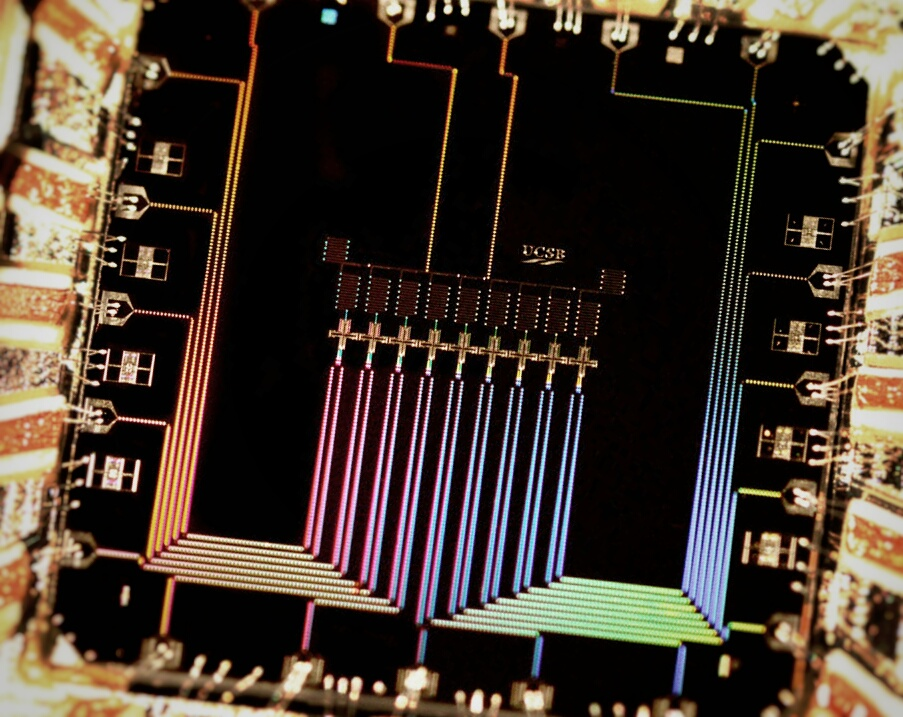
\includegraphics[width=\linewidth]{gfx/Linear9XmonSurfaceCode}
     \caption{\footnotesize Martinis group website, UCSB}
    \end{figure}

 \end{columns}


\end{frame}

% \begin{frame}{Quantum Speed-Up}
%  
%  \structure{Hope/Expectation:} Many problems can be solved faster on a quantum computer.
%  
%  \begin{columns}
%   \column{0.5\linewidth}
%   \structure{Evidence:} \Eg~Shor's algorithm
%   
%   \column{0.5\linewidth}
%     \begin{figure}
%      \centering
%      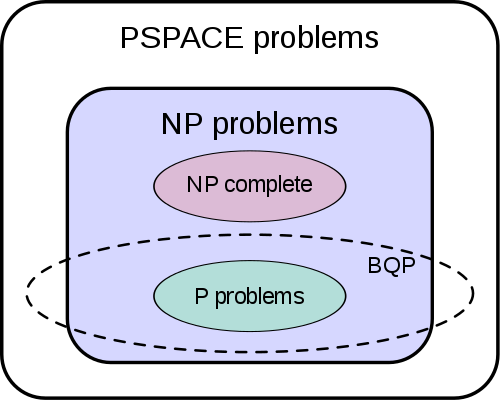
\includegraphics[width=\linewidth]{gfx/BQP_complexity_class_diagram}
%      \caption{\footnotesize Wikipedia/BQP}
%     \end{figure}
%  \end{columns}
%  
% \end{frame}

% \begin{frame}{Quantum Algorithms}
% 
% \structure{Examples:} Grover search algorithm, Shor's factoring algorithm, \dots
% 
% \alert{But: This list is not that long!}
%  
% \end{frame}
